\documentclass[handout,nooutcomes]{ximera}
\usepackage{booktabs}
%% handout
%% space
%% newpage
%% numbers
%% nooutcomes

\renewcommand{\outcome}[1]{\marginpar{\null\vspace{2ex}\scriptsize\framebox{\parbox{0.75in}{\begin{raggedright}P\arabic{problem} Outcome: #1\end{raggedright}}}}}

\renewenvironment{freeResponse}{
\ifhandout\setbox0\vbox\bgroup\else
\begin{trivlist}\item[\hskip \labelsep\bfseries Solution:\hspace{2ex}]
\fi}
{\ifhandout\egroup\else
\end{trivlist}
\fi}

\newcommand{\RR}{\mathbb R}
\renewcommand{\d}{\,d}
\newcommand{\dd}[2][]{\frac{d #1}{d #2}}
\renewcommand{\l}{\ell}
\newcommand{\ddx}{\frac{d}{dx}}
\everymath{\displaystyle}
\newcommand{\dfn}{\textbf}
\newcommand{\eval}[1]{\bigg[ #1 \bigg]}


\title{Breakout Session 15: Related Rates (Part II) and Extrema}

\begin{document}
\begin{abstract}
  \textbf{A look back:} In the previous (February 25, 2016) Breakout Session you were introduced to related rates~---~an important application of derivatives.

  \textbf{Overview:} In today's (March 1, 2016) Breakout Session you'll practice locating absolute extrema and local extrema of continuous functions on closed intervals.
  
  \textbf{A look ahead:} In the next (March 3, 2016) Breakout Session you'll learn how the sign of the first and second derivatives influence the shape of the graph of the function.
\end{abstract}
\maketitle

\section{Learning Outcomes}
\label{section:learning-outcomes}
The following outcomes are \emph{not an exhaustive} list of the skills you will need to develop and integrate for demonstration on quizzes and exams.
This list is meant to be a starting point for conversation (with your Lecturer, Breakout Session Instructor, and fellow learners) for organizing your knowledge and monitoring the development of your skills.

\begin{itemize}
  \item 
    Identify word problems as related rates problems.
  \item 
    Translate word problems into mathematical expressions.
  \item 
    Calculate derivatives of expressions with multiple variables implicitly.
  \item 
    Understand the process of solving related rates problems.
  \item
    Solve related rates word problems.
  \item
    Define a critical point. 
  \item 
    Find critical points.
  \item
    Find the absolute max or min of a continuous function on a closed interval.
  \item
    Solve basic word problems involving maxima or minima. 
  \item
    Compare and contrast local and absolute maxima and minima. 
  \item
    Identify situations in which an absolute maximum or minimum is guaranteed.
\end{itemize}
\newpage

\begin{image}
 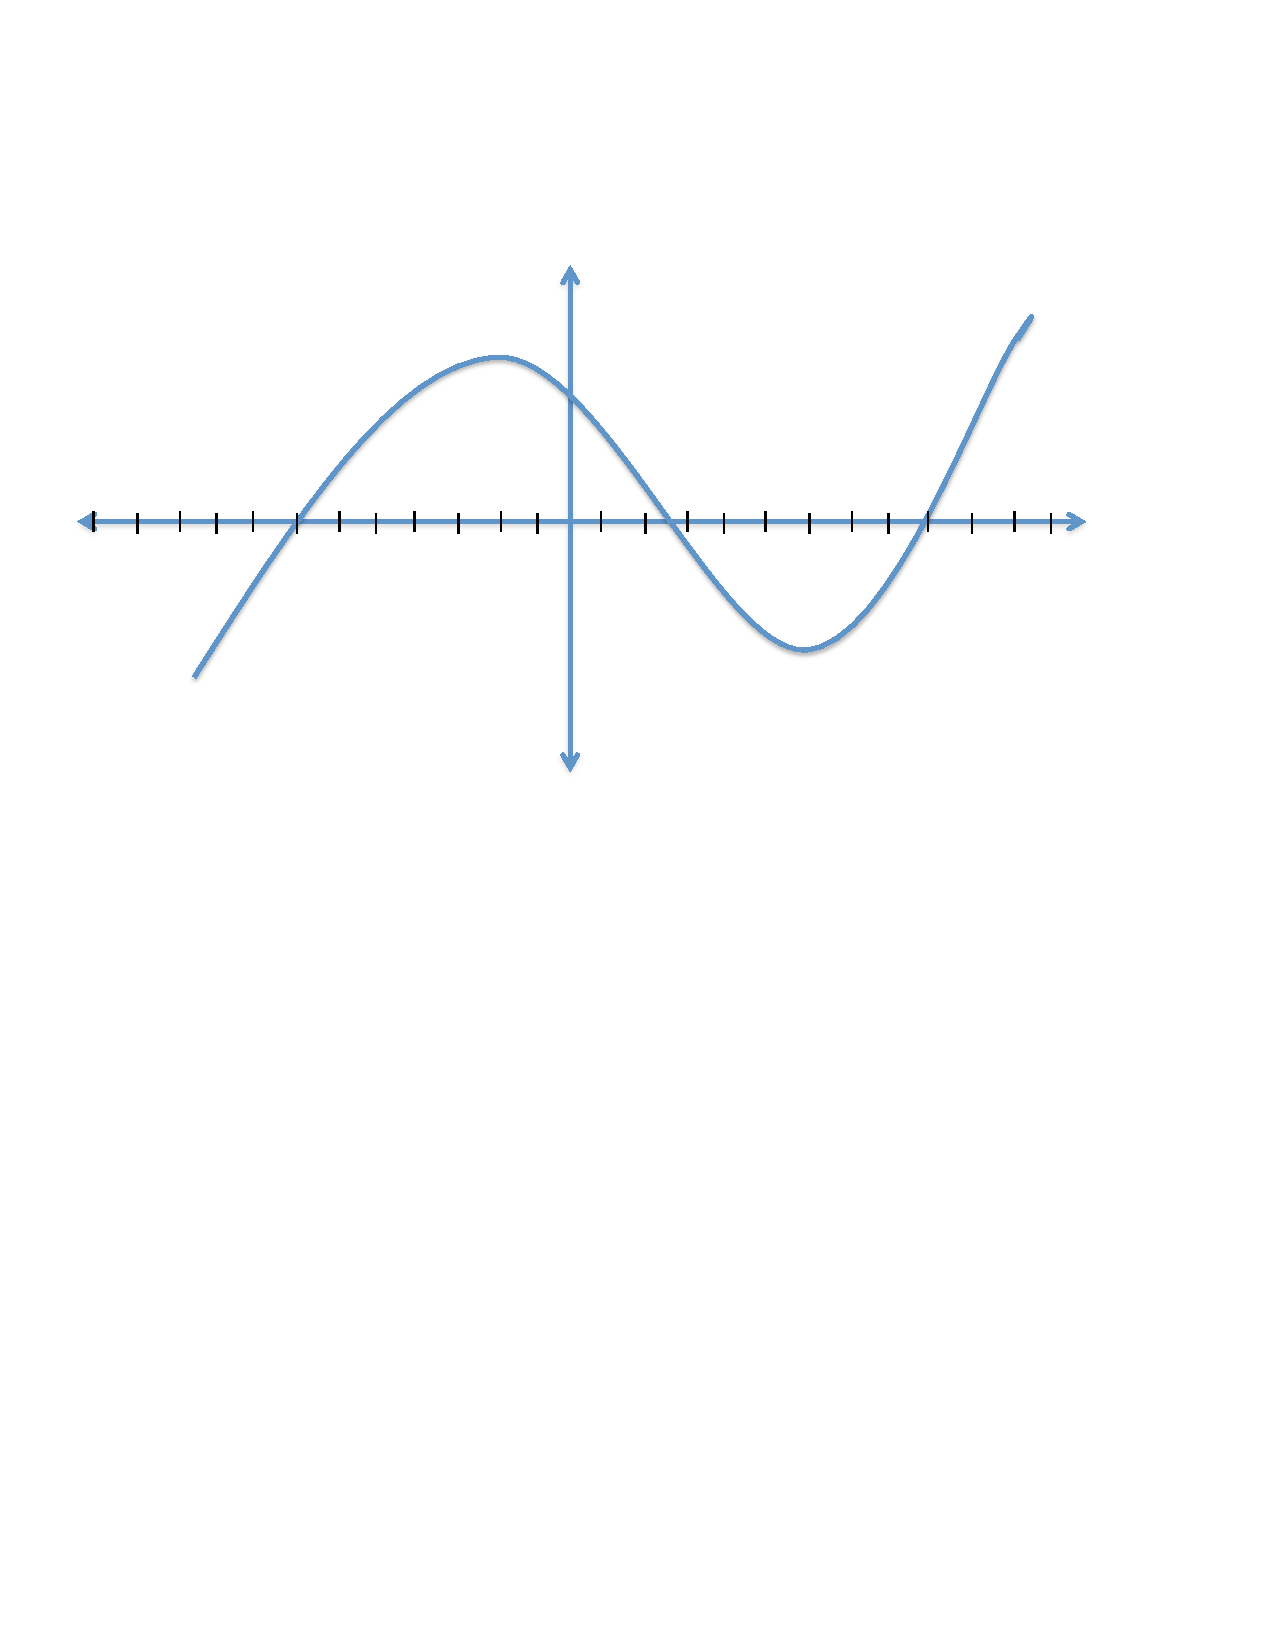
\includegraphics[trim= 220 480 250 90]{Images/Figure2.pdf}
\end{image}

\begin{problem}
  A right cone has fixed slant height (see figure) of 9 ft.
  The cone's height is shrinking at a rate of 0.5 ft/sec.
  At what rate is the area of the base changing when the height is 6 ft?
  (Be sure to label the figure.)
  \begin{center}
    \begin{image}
      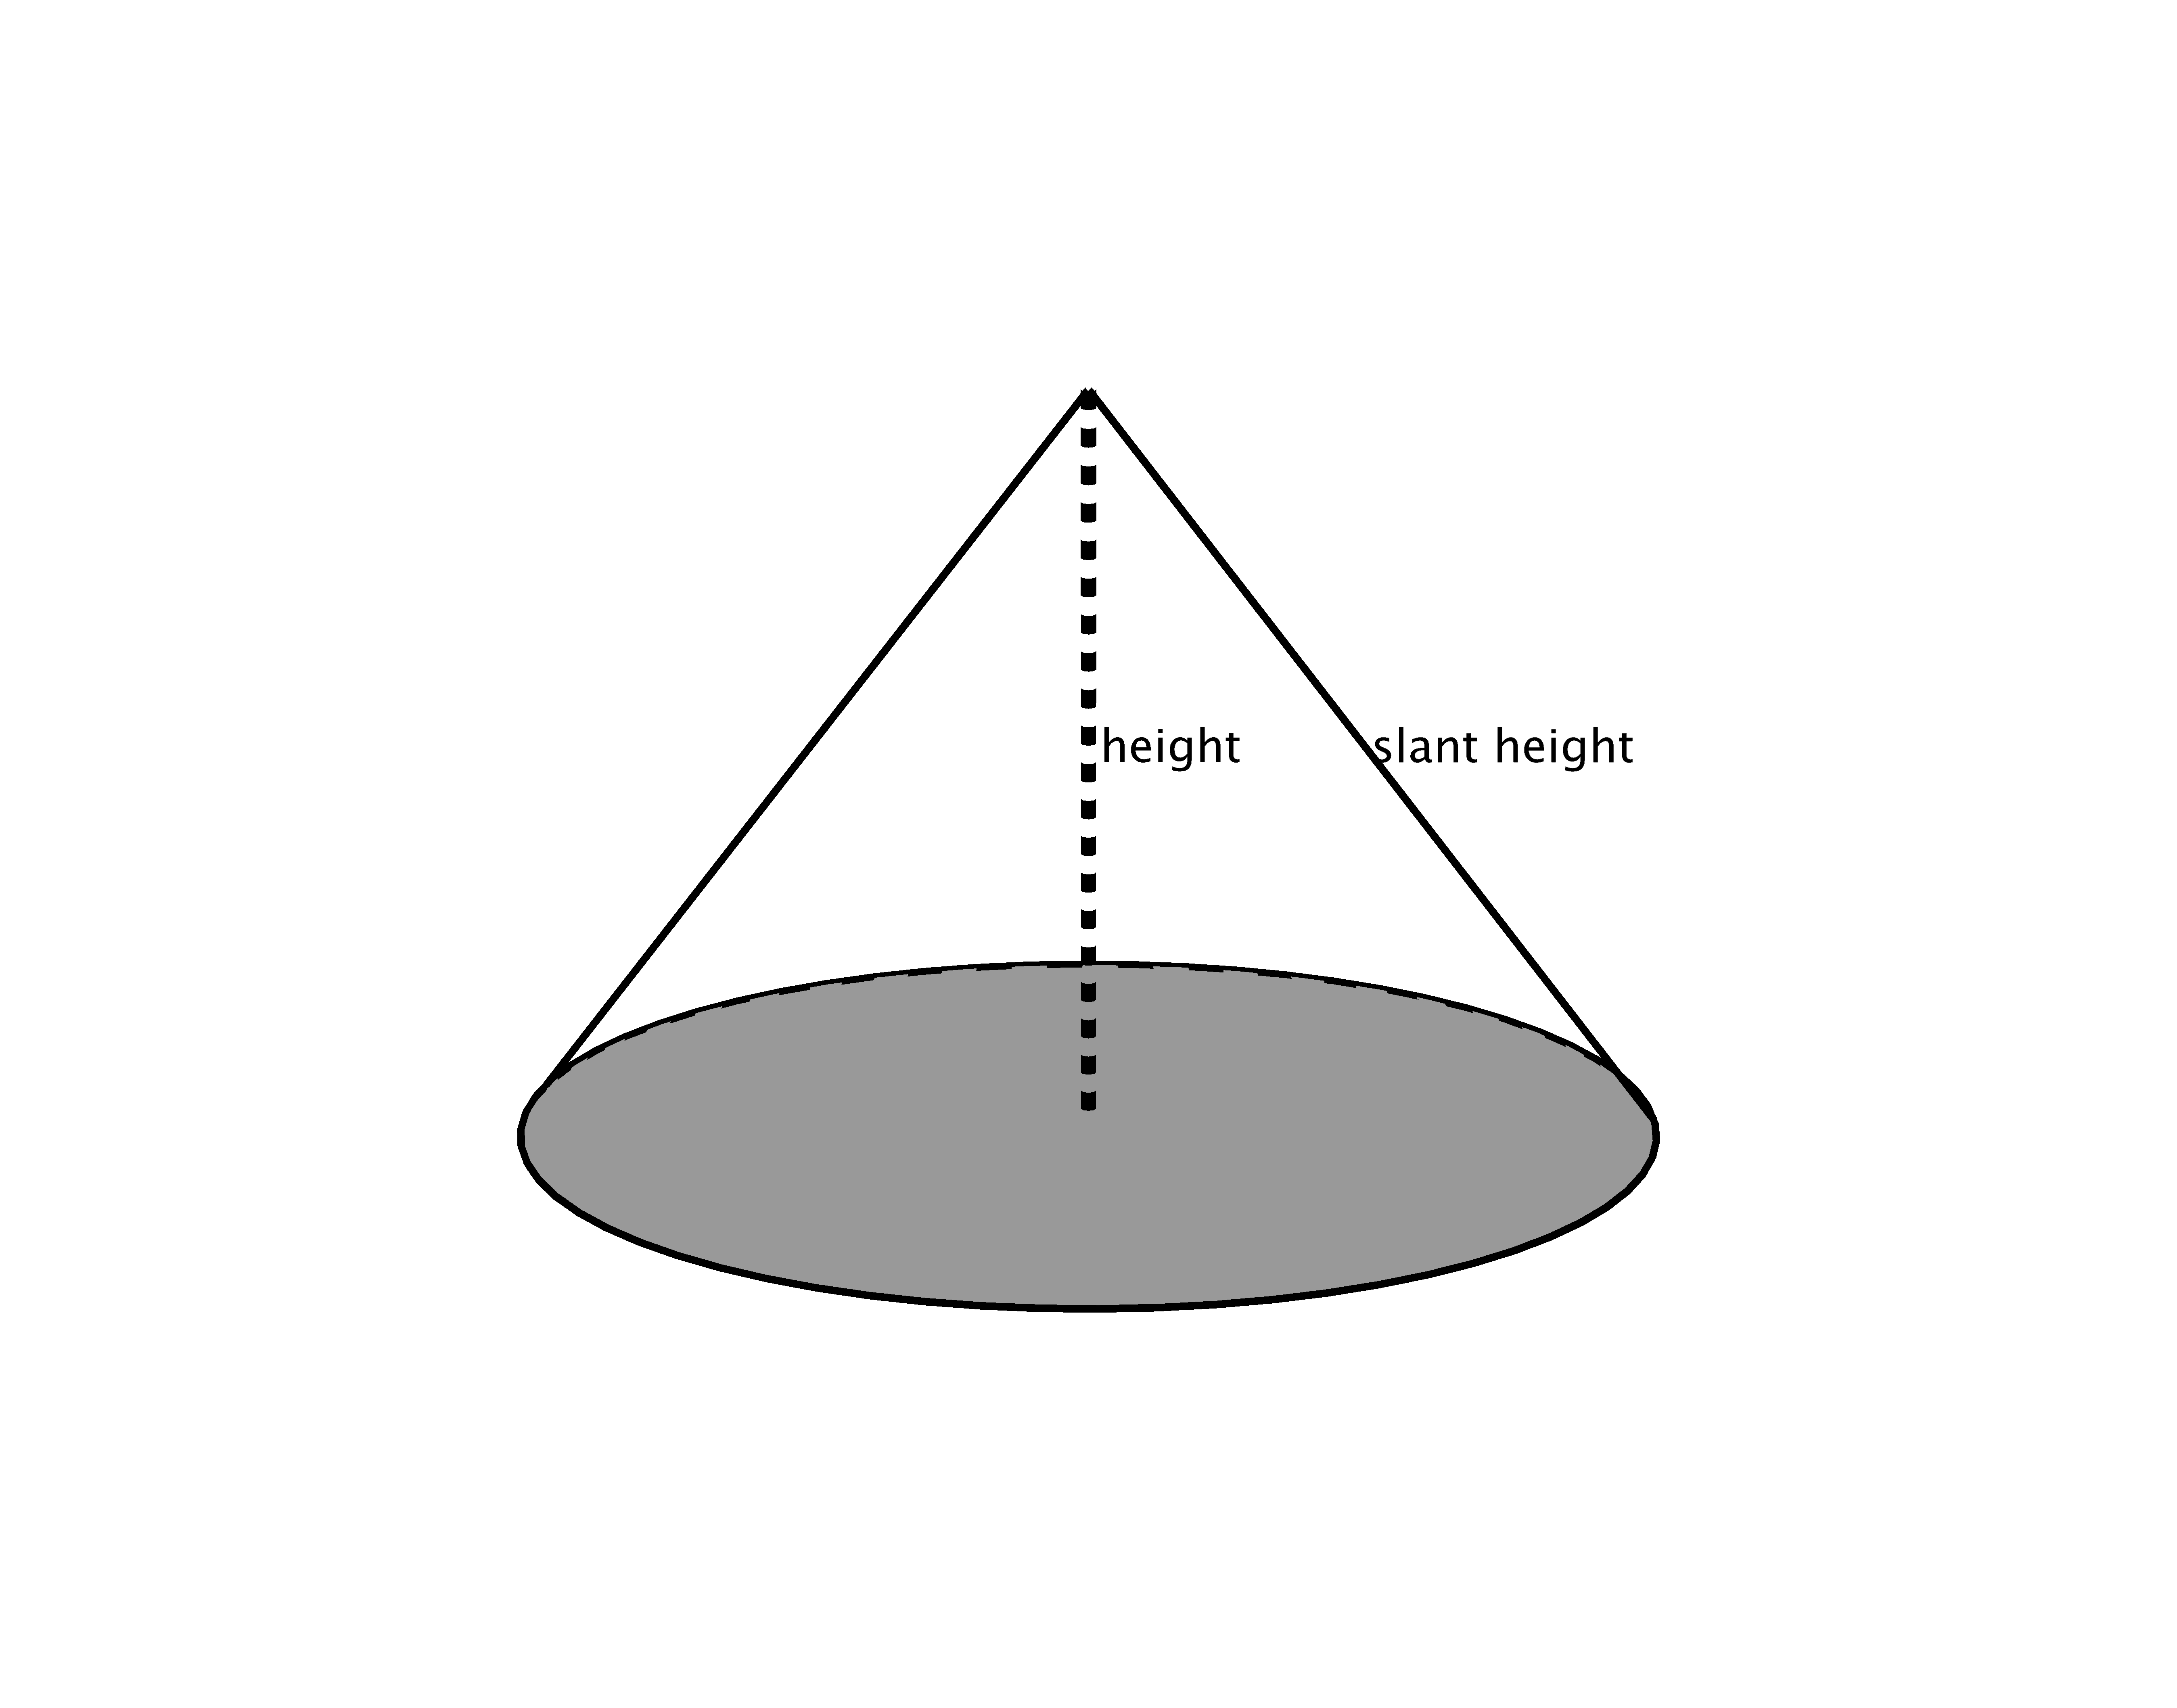
\includegraphics[scale = 0.3]{Images/Cone.png}
    \end{image}
  \end{center}
\end{problem}

\begin{problem}
A swimming pool is 20 feet long and has transverse cross sections which look like the figure below.   If the pool is being filled at a rate of 0.8 cubic feet per minute, how fast is the water level rising when the depth of the water is 3 feet? 
	\begin{image}
	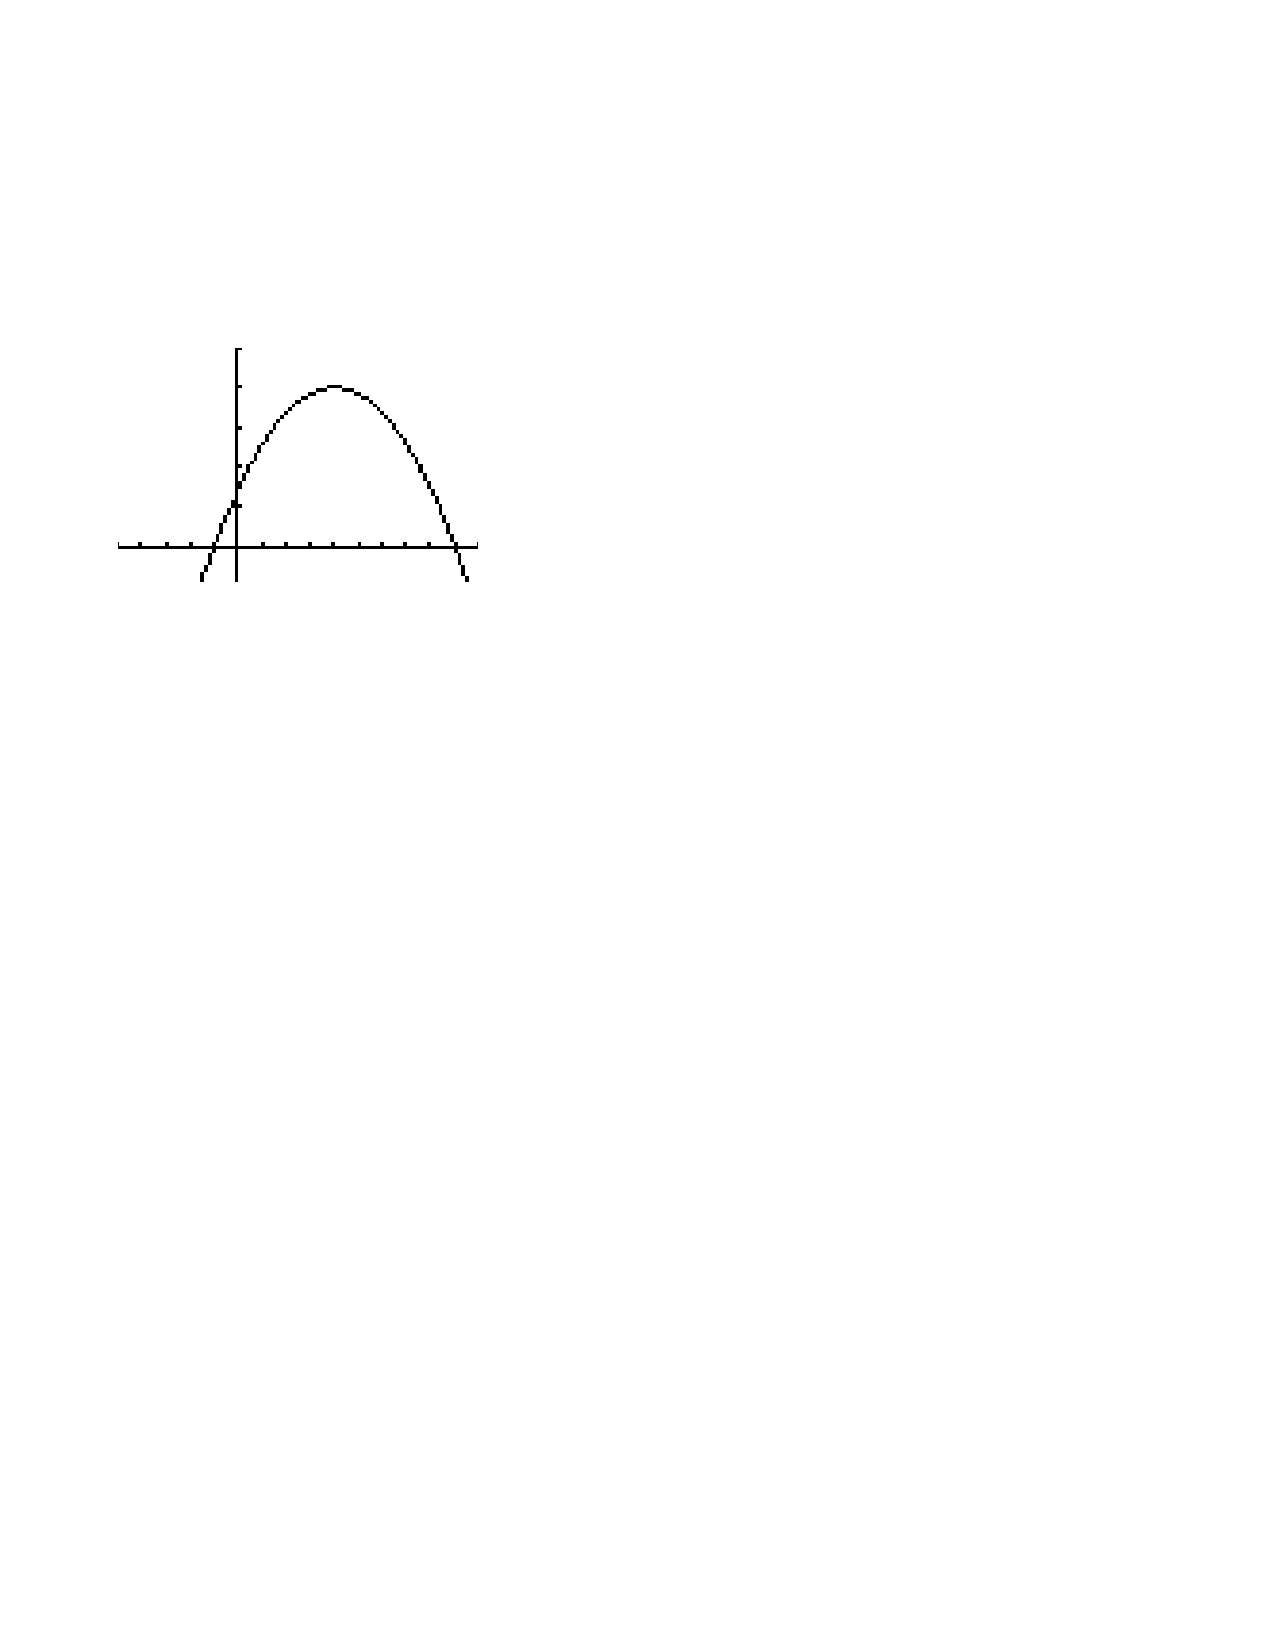
\includegraphics[trim= 100 500 250 170]{Images/Figure4.pdf}
	\end{image}
	
		\begin{freeResponse}
		Let $V$ denote the volume and $h$ denote the height of the water in the pool.  We are given that the pool is being filled at a rate of $0.8$ cubic feet per minute, and so $\dd[V]{t} = \frac{4}{5} \frac{ft^3}{min}$.  We want to find $\dd[h]{t}$ at the instant in time when $h=3 ft$.  Since the height that we care about is below the height $h=6 ft$ where the pool changes shape, we only need to worry about the shape of the bottom of the pool.  This portion of the pool looks like:
		
		\begin{image}
		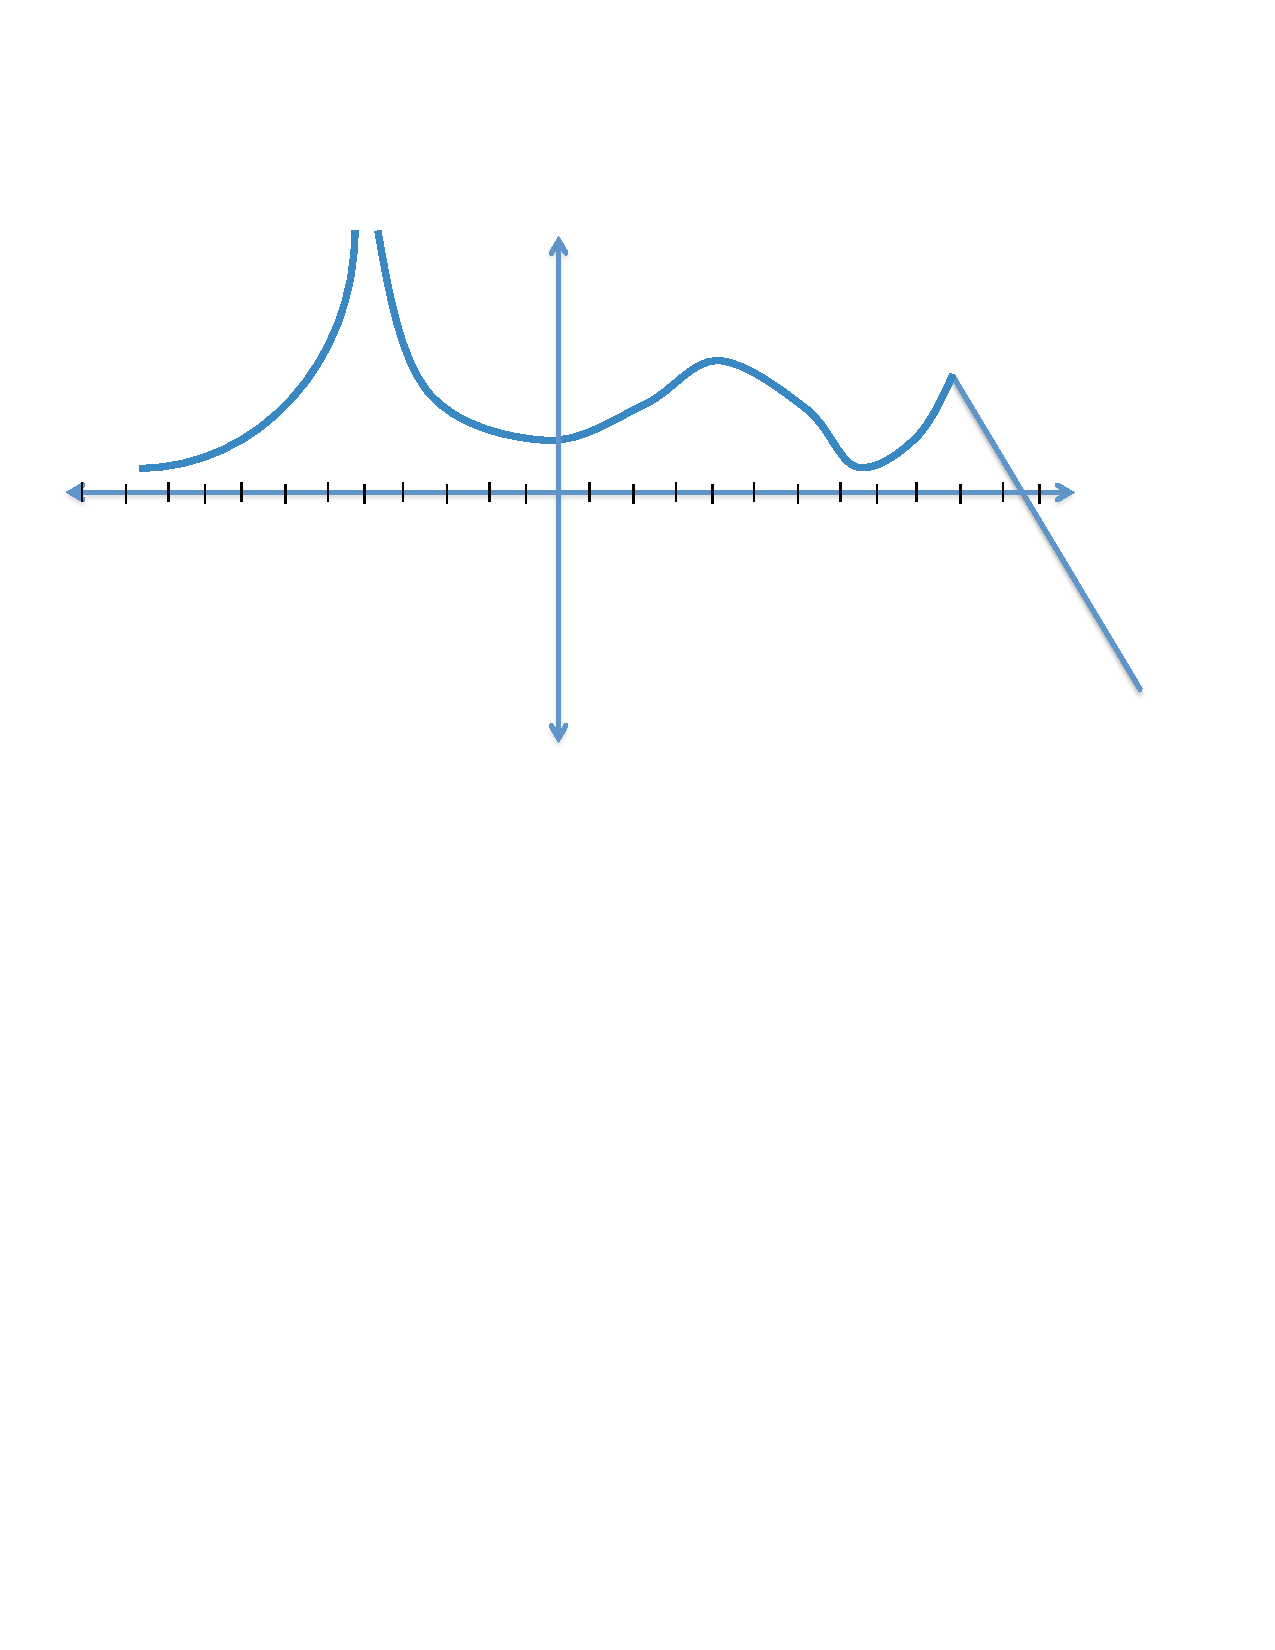
\includegraphics[trim= 100 500 250 200]{Images/Figure5.pdf}
		\end{image}
		
		Observe that the volume of the water in the pool is
		\begin{equation}\label{Vprob2}
		V = 20 \left( 14h + 2 \left( \frac{1}{2} xh \right) \right) = 20 \left( 14h + xh \right)
		\end{equation}
		where $x$ is as in the picture above, and the 20 is due to the length of the pool.  
		
		We could attempt to solve for $\dd[h]{t}$ by differentiating equation \ref{Vprob2} with respect to time, but the problem is that we do not know $\dd[x]{t}$.  So we need to use the geometry of the problem to write $x$ as a function of $h$.  And we do that here by using similar triangles.  Notice that $\frac{x}{h} = \frac{3}{6} = \frac{1}{2}$, and so $x = \frac{1}{2} h$.  Substituting this into equation \ref{Vprob2} yields:
		$$ V = 20 \left( 14h + \frac{1}{2} h^2 \right) $$
		
		Now we differentiate with respect to time, substitute, and solve for $\dd[h]{t}$:
		$$ \dd[V]{t} = 20 \left( 14 \dd[h]{t} + h \dd[h]{t} \right) $$
		$$ \frac{4}{5} = 20 \left( 14 \dd[h]{t} + 3 \dd[h]{t} \right) $$
		$$ \frac{4}{5} = 340 \dd[h]{t} $$
		$$ \dd[h]{t} = \frac{4}{5 \cdot 340} \frac{ft}{min} = \frac{1}{5 \cdot 85} \frac{ft}{min} = \frac{1}{425} \frac{ft}{min}. $$
		\end{freeResponse}
\end{problem}

\begin{problem}
  Serena Scaralet Gray is changing the oil in her car, the Buckeye mobile.
  She adds the new oil using a funnel (an inverted cone) with height 12 cm and radius 10 cm.
  The oil drains out of the funnel at a rate of 3 $\mbox{cm}^3/\mbox{s}$.
  What is the rate of change of the oil's depth when the oil depth is 4 cm?
\end{problem}


\begin{problem}
For each of the points identified on the graph below, determine if the point is a critical point, a local max or min, and/or an absolute max or min.

	\begin{center}
	\begin{image}
	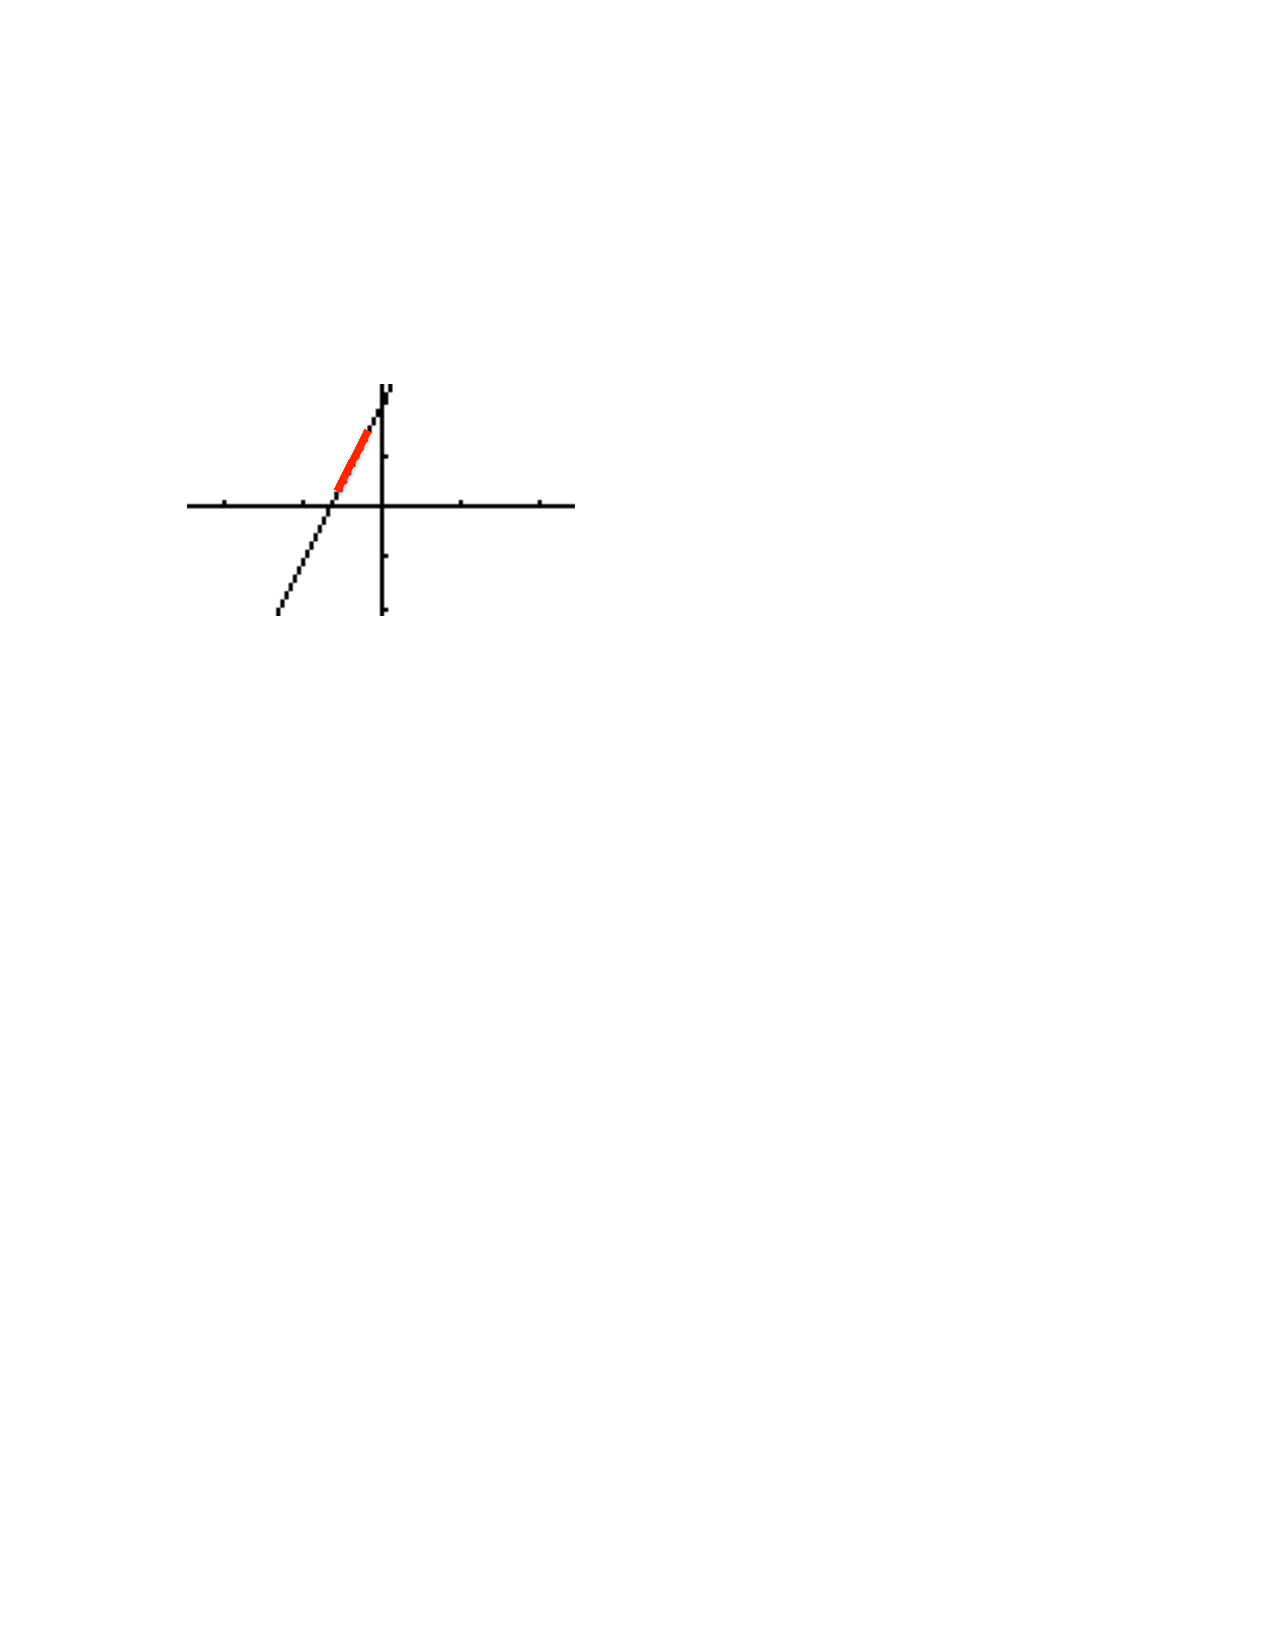
\includegraphics[trim= 20 430 250 200]{Images/Figure8.pdf}
	\end{image}
	\end{center}	
	
		\begin{freeResponse}
(a) This point is the absolute minimum.

(p) This point is a critical point and is the absolute maximum.  It is also a local maximum.

(q) This point is a critical point and is a local minimum.

(r) This point is a critical point and is a local maximum.

(s) The derivative does not exist because the function has a corner.  This point is a critical point and is a local minimum.

(t) This point is a critical point but is not a local maximum or minimum.

(b) This point is not an absolute or local max or min.
		\end{freeResponse}	
		
\end{problem}

\begin{problem}
All rectangles with an area of $64$ have a perimeter given by $P(x)=2x+\frac{128}{x}$, where $x$ is the length of one side of the rectangle.  Find the absolute minimum value of the perimeter function.  What are the dimensions of the rectangle with minimum perimeter?   
		\begin{freeResponse}
		First note that the domain for $P(x)$ is $(0,\infty)$.  To find the critical points of $P$, we solve the equation $P'(x) = 0$:
		$$ P'(x) = 2 - \frac{128}{x^2} := 0 $$
		$$ \frac{128}{x^2} = 2 $$
		$$ 2x^2 = 128 $$
		$$ x^2 = 64 $$
		$$ x = \pm 8 $$
		but since we must have $x>0$, our only critical point is $x=8$.  Notice that for $x \in (0,8)$, $P'(x) < 0$, and for $x \in (8, \infty)$, $P'(x) > 0$.  Thus $x=8$ is a local minimum by the first derivative test.  But since $P$ is decreasing over the entire interval $(0,8)$ and increasing over the entire interval $(8,\infty)$, $x=8$ must be an absolute minimum.
		
		Hence, the absolute minimum perimeter is $P(4) = 16 + \frac{128}{8} = 16 + 16 = 32$.  Since the dimensions of such a rectangle are $8 \times 8$, a rectangle of minimum perimeter is a square.
		\end{freeResponse}
			
\end{problem}			



\section{Extra Problems for Personal Practice}


\begin{problem}
An oil spill is being cleaned up by the deployment of bacteria that consume the oil at 3 cubic feet per hour.  The oil spill itself is modeled in the form of a very thin cylinder with height $h$ being the thickness of the oil slick (see the picture below).  Suppose at some moment in time, the height is decreasing at 0.0005 feet per hour, the thickness of the slick is 0.007 feet, and the cylinder is 900 feet in diameter.  At what rate is the area covered by the slick changing at that moment (that is, the area of the base disc of the cylinder)?
	\begin{image}
	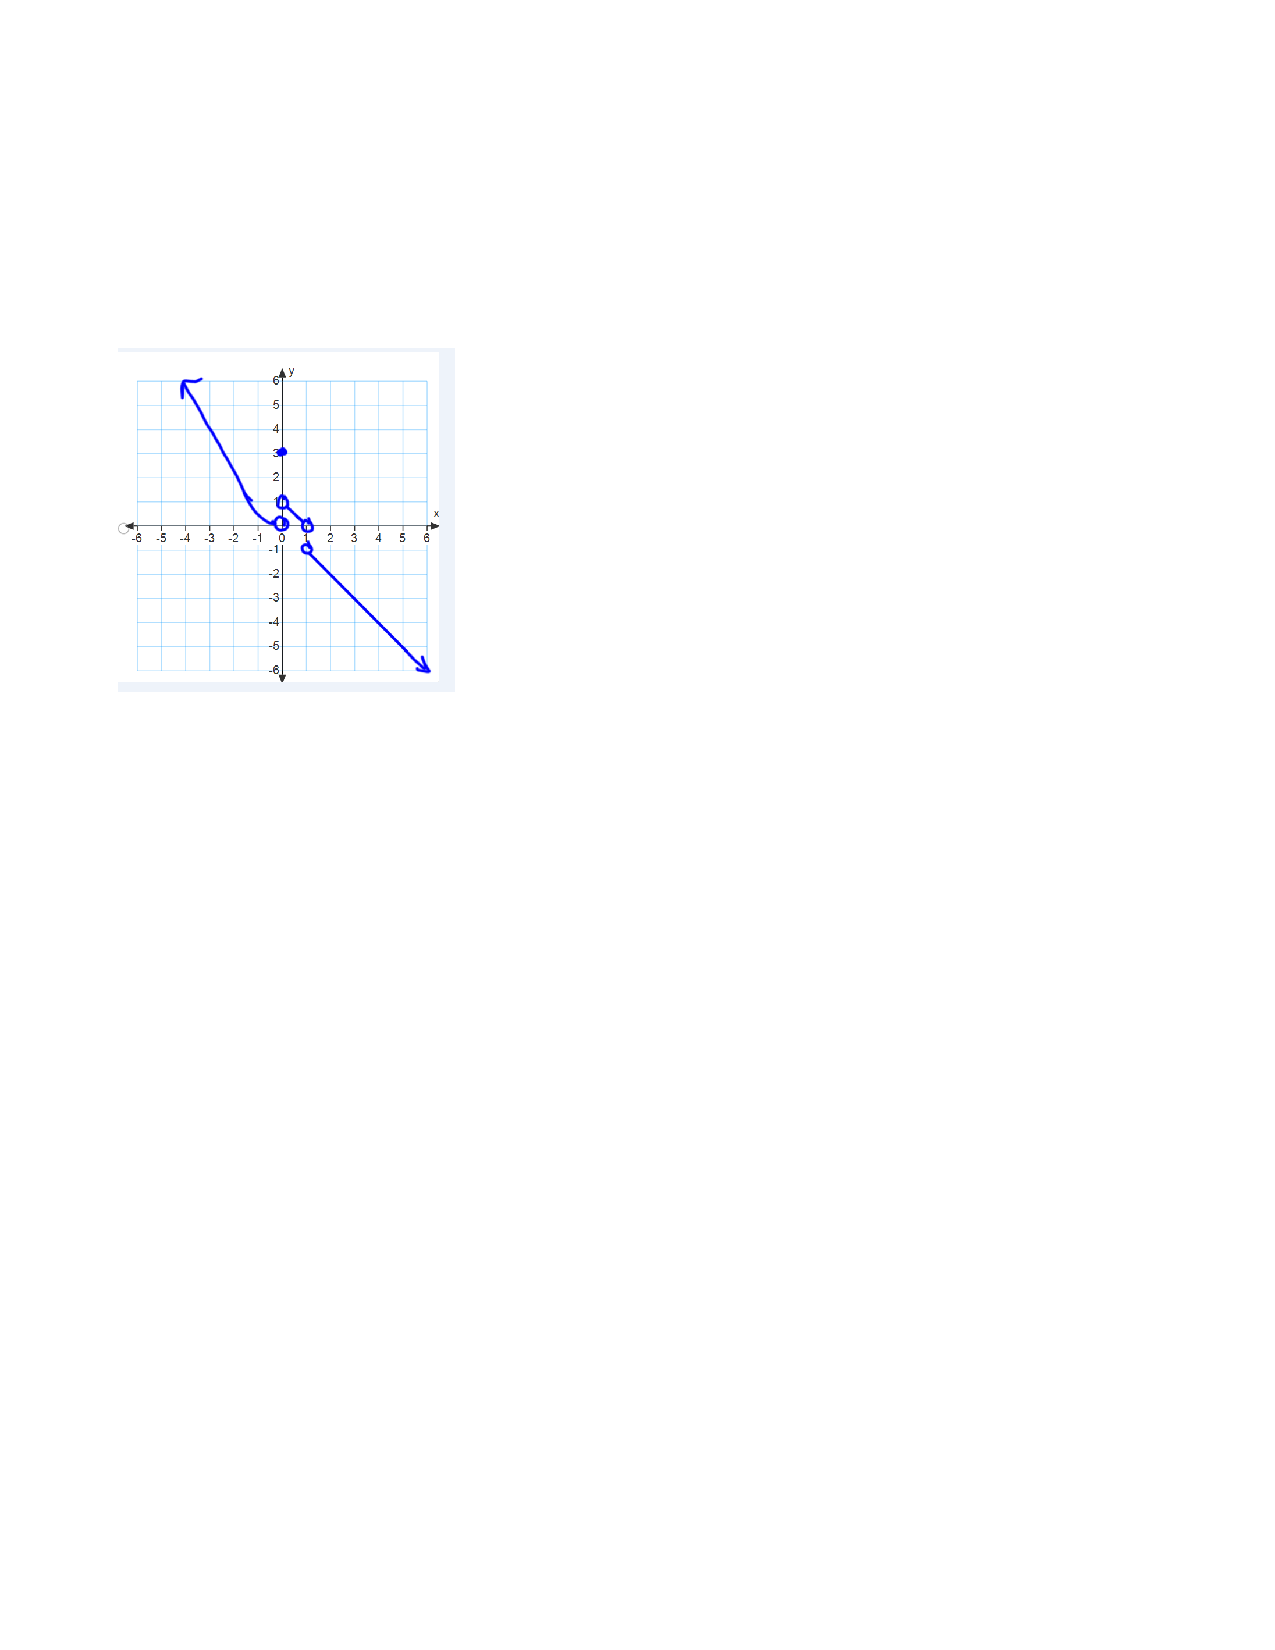
\includegraphics[trim= 100 520 250 220]{Images/Figure3.pdf}
	\end{image}
	
		\begin{freeResponse}
		Let $V$ denote the volume, $A$ denote the area of the base, $h$ denote the height (or thickness), and $r$ denote the radius of the oil slick.  Note that the first piece of information that we are given is that $\dd[V]{t} = -3 \, \frac{ft^3}{hr}$.  
		
		Let $t_0$ denote the instant in time that we are concerned about.  Then at time $t_0$ we are also given that:
		$$ \dd[h]{t} = \left( -5 \times 10^{-4} \right) \frac{ft}{hr}  \qquad  h = \left( 7 \times 10^{-3} \right) ft  \qquad  r = \left( 4.5 \times 10^2 \right) ft $$
		and the problem asks us to find $\dd[A]{t}$ at time $t_0$.  
		
		Since $A = \pi r^2$, we have that $\dd[A]{t} = 2 \pi r \dd[r]{t}$.  So at time $t_0$ we have that $\dd[A]{t} = 900 \pi \dd[r]{t}$.  Unfortunately, we are not given $\dd[r]{t}$ at time $t_0$, and so our goal now is to find this.
		
		Since $V = \pi r^2 h$, we can use the product rule to compute
		\begin{equation}\label{dVdtprob1}
		\dd[V]{t} = \pi \left( 2r \dd[r]{t} h + r^2 \dd[h]{t} \right)
		\end{equation}
		
		Using all of our known quantities, we can plug into equation \ref{dVdtprob1} and solve for $\dd[r]{t}$ at time $t_0$:
		$$ -3 = \pi \left( 2(450)(7 \times 10^{-3}) \dd[r]{t} + (4.5 \times 10^2)^2(-5 \times 10^{-4}) \right) $$
		$$ -3 = \pi \left( 900(7 \times 10^{-3}) \dd[r]{t} + (20.25 \times 10^4) (-5 \times 10^{-4}) \right) $$
		$$ -3 = 6.3 \pi \dd[r]{t} -101.25 \pi $$
		$$ \dd[r]{t} = \frac{101.25 \pi - 3}{6.3 \pi} $$
		
		Thus, we solve
		$$ \dd[A]{t} = 900 \pi \cdot \frac{101.25 \pi - 3}{6.3 \pi} \, \frac{ft^2}{hr} = 900 \left( \frac{101.25 \pi - 3}{6.3} \right) \, \frac{ft^2}{hr} $$
		
		%another solution
		\dfn{Another Solution}
		
		Here is a very nice, but less obvious, solution to this problem.
		$V = \pi r^2 h = Ah$.  So 
		$$ \dd[V]{t} = \dd[A]{t} h + A \dd[h]{t} = \dd[A]{t} h + \pi r^2 \dd[h]{t}$$
		and thus
		$$ -3 = (7 \times 10^{-3}) \dd[A]{t} + \pi \cdot 450^2 \cdot (-5 \times 10^{-4}) $$
		$$ -3 = (7 \times 10^{-3}) \dd[A]{t} - 101.25 \pi  $$
		$$ \dd[A]{t} = \frac{101.25 \pi - 3}{7 \times 10^{-3}} \, \frac{ft^2}{hr} $$
		\end{freeResponse}
\end{problem}

\begin{problem}
  Determine whether the following statements are true or false and
  give either an explanation or a counterexample.

  \begin{enumerate}
	

  \item The function $f(x) = \sqrt{x}$ has a local maximum on the
    interval $[0,1]$.
    \begin{freeResponse}
      False.  Since $\sqrt{x}$ is increasing over the entire region
      $[0,1]$, the only candidate for a local maximum would be $x=1$.
      But by definition, endpoints are never local extrema.  So
      $f(x) = \sqrt{x}$ has no local maximum on the interval $[0,1]$.
    \end{freeResponse}
		
		
		

  \item If a function has an absolute maximum value on a closed
    interval, then the function must be continuous on that closed
    interval.
    \begin{freeResponse}
      False.  Consider the following graph for a counterexample.  The
      function has an absolute maximum on the interval $[2,10]$, but
      it is not continuous over the entire interval.
		
      \begin{image}
        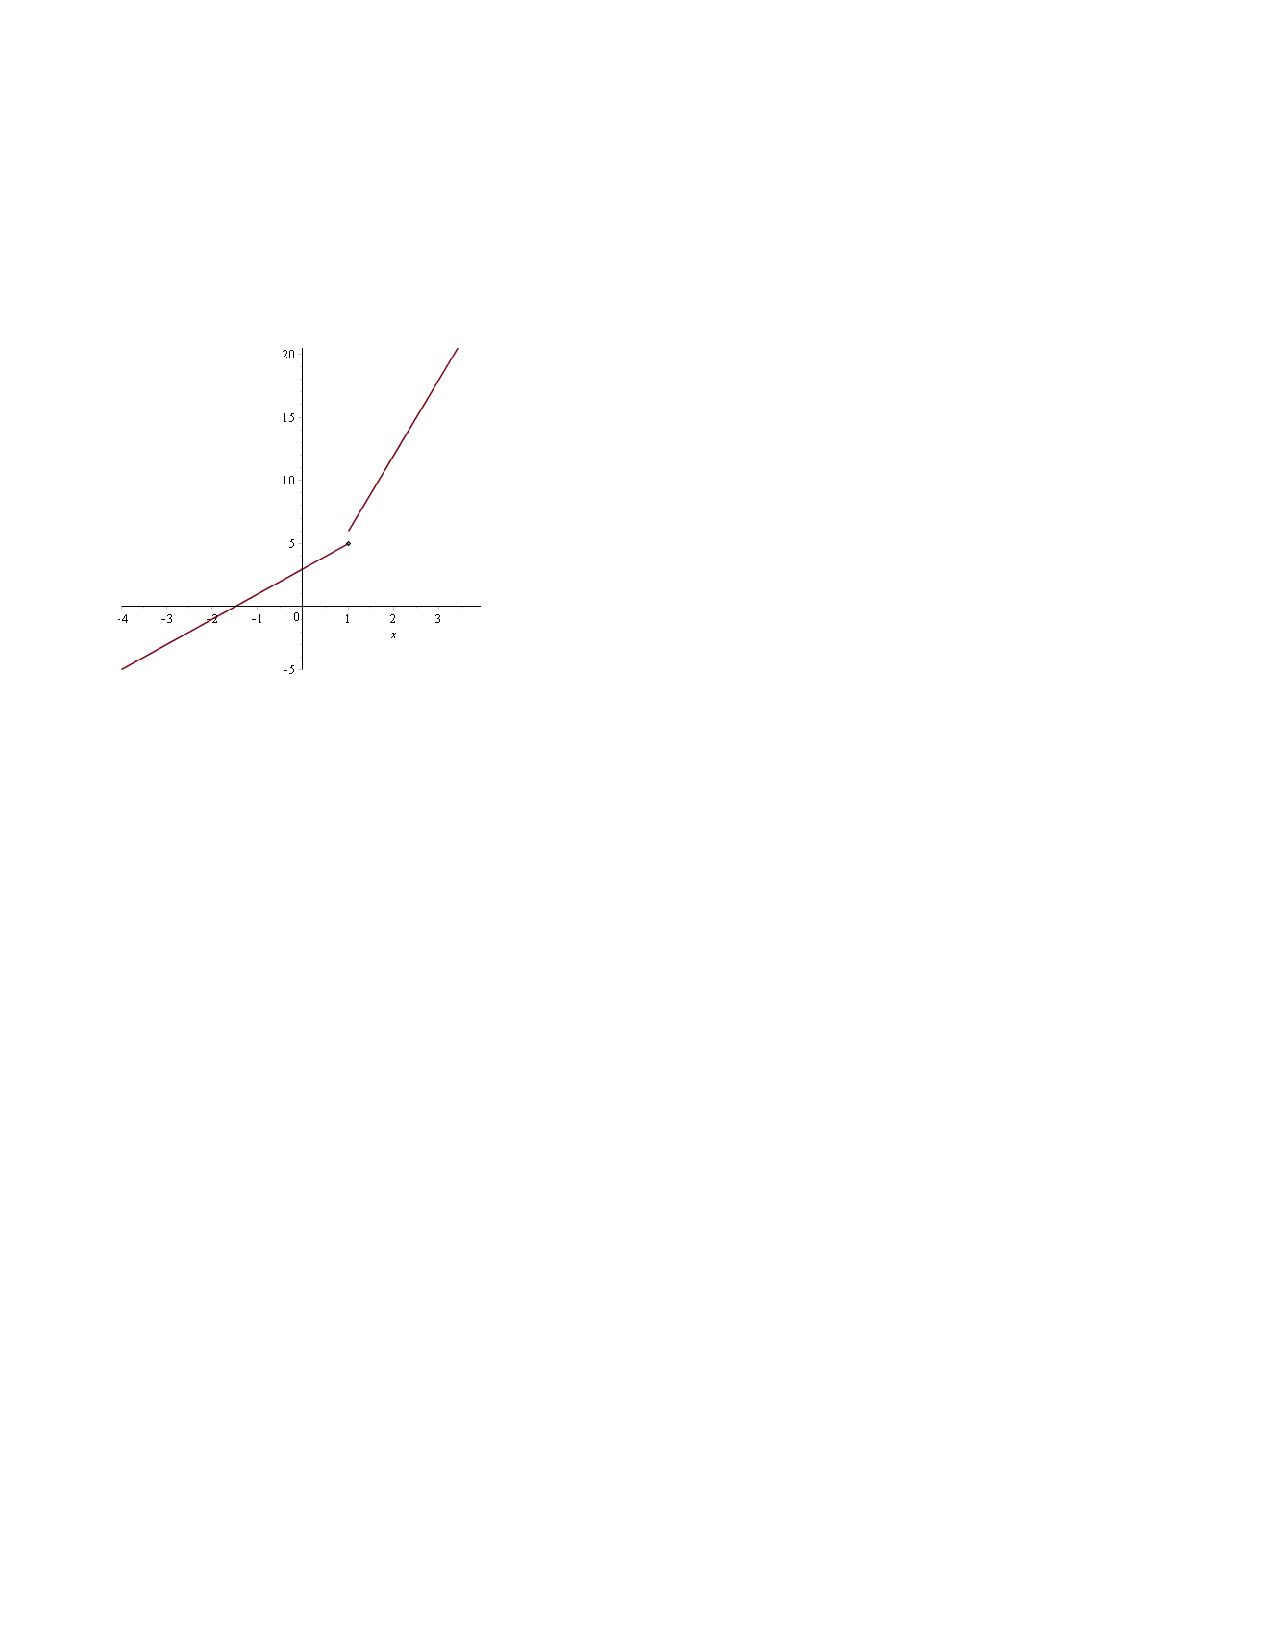
\includegraphics[trim= 170 380 250 180]{Images/Figure6.pdf}
      \end{image}
		
      It is worth noting though that the converse to the original
      statement is true.  i.e., if a function is continuous on a
      closed interval then it obtains an absolute maximum value on
      that closed interval.

    \end{freeResponse}
		
		
		

  \item If $f'(2)=0$, then $x=2$ is either a local maximum or local
    minimum of $f$.
    \begin{freeResponse}
      False.  Consider $f(x) = (x-2)^3$.  $f'(x) = 3(x-2)^2$, and so
      $f'(2) = 0$.  But we can see by looking at the graph of $f$ that
      $x=2$ is not a local extreme value for $f$.
      \begin{image}
        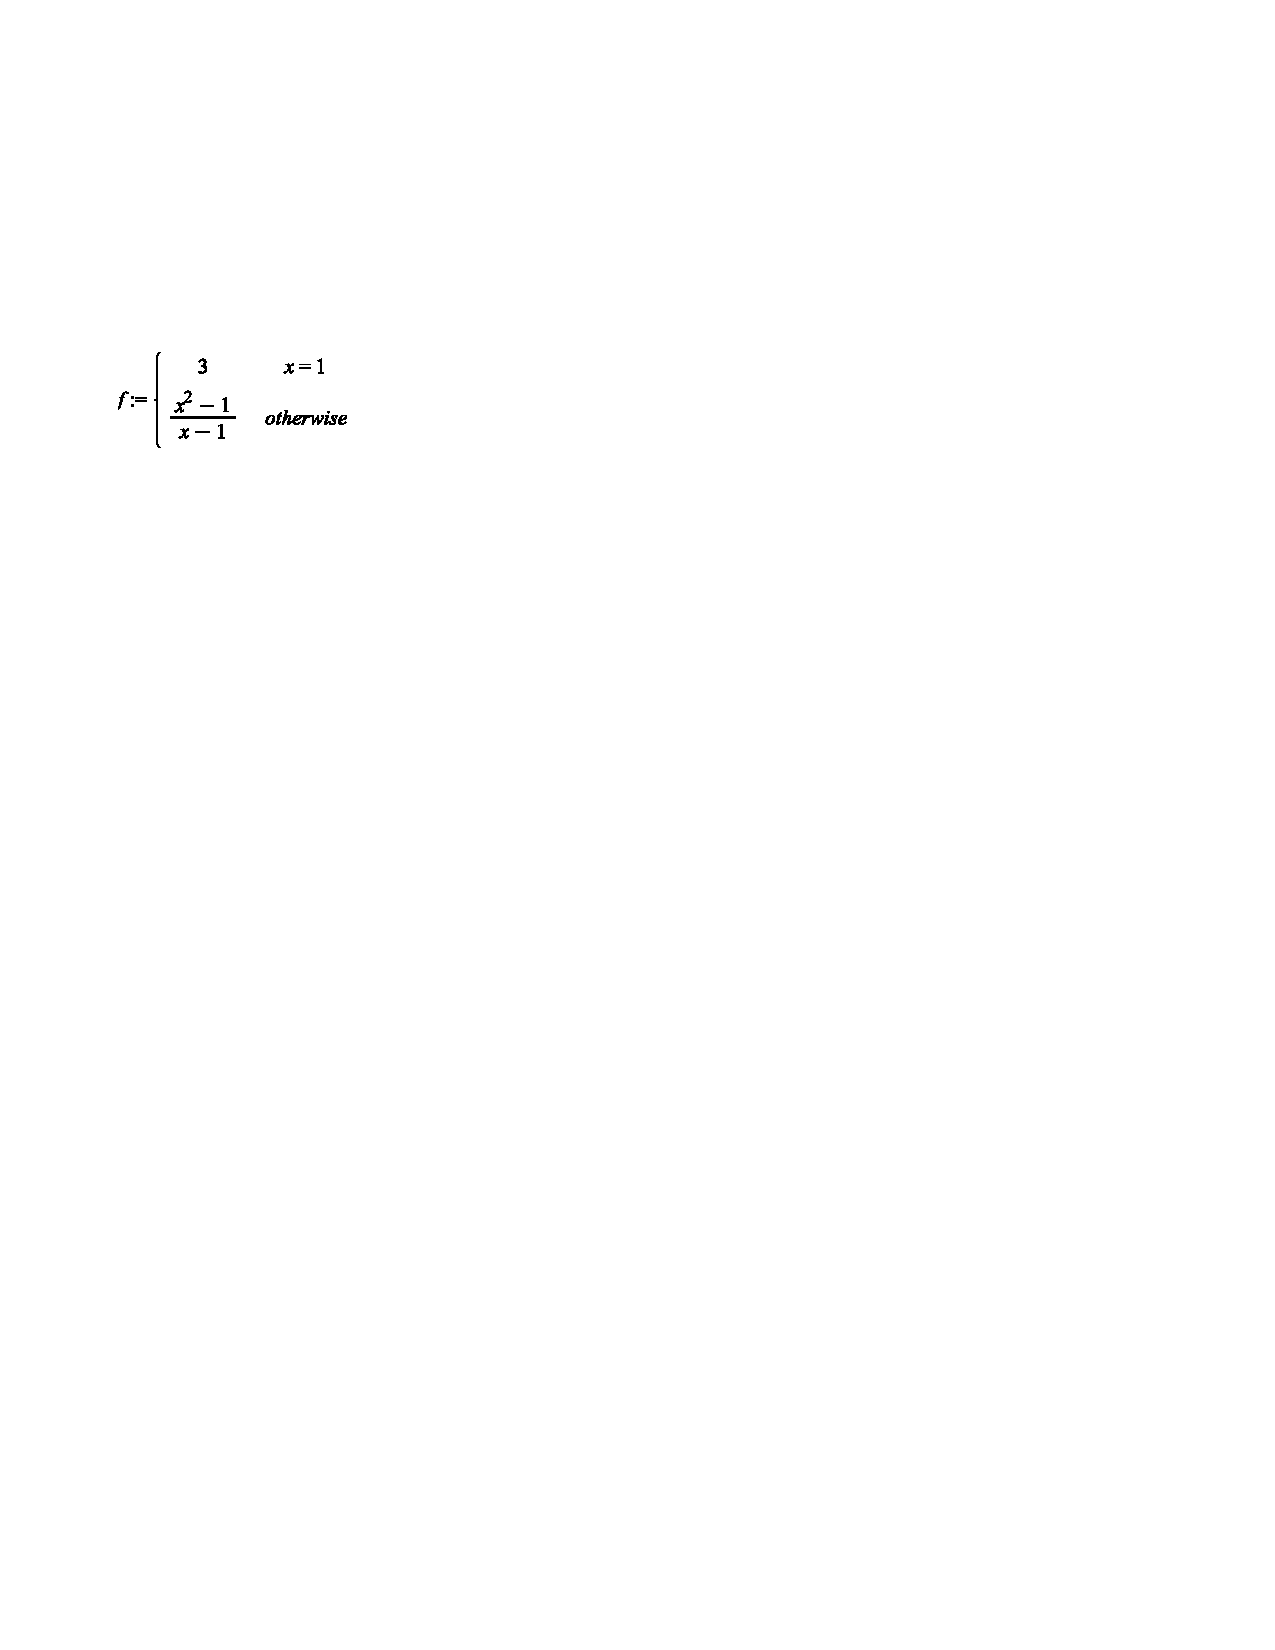
\includegraphics[trim= 100 430 250 180]{Images/Figure7.pdf}
      \end{image}
    \end{freeResponse}
		
		
		

  \item Absolute extreme values on a closed interval always occur at a
    critical point or an endpoint of the interval.
    \begin{freeResponse}
      True.  The pretty much follows directly from the Local Extreme
      Value Theorem.  All absolute extrema must either be local
      extrema or endpoints.  And by the Local Extreme Value Theorem,
      all local extrema must be critical points of the function.
    \end{freeResponse}
		
		
		
    % part e
  \item If $x=3$ is in the domain of $f$ and if $f'(3)$ does not
    exist, then $x=3$ is a critical point of $f$.
    \begin{freeResponse}
      Technically this is false, but morally it is true.  If the
      domain of $f$ is some closed interval with $3$ as an endpoint,
      then $3$ is in the domain of $f$ and $f'(3)$ does not exist
      (since one of the sided limits of the derivative will not
      exist).  Certainly $x=3$ may not be a critical point of $f$, for
      example, consider the function $f(x) = x$ with domain $[0,3]$.
      But this whole setup is a technicality because we had to
      restrict the natural domain of the function.  If $f'(3)$ does
      not exist and $x=3$ is an \emph{interior} point of the domain of
      $f$, then $x=3$ is a critical point of $f$.
    \end{freeResponse}
  \end{enumerate}
\end{problem}


\begin{problem}
Find the critical points of $f$ on the given interval, and determine the absolute extreme values of $f$ on the interval.
		\begin{enumerate}
		
			%part a
			\item  $f(x) = x \sqrt{2-x^2}$ on $[ -\sqrt{2}, \sqrt{2} ]$.
				
				\begin{freeResponse}
				First note that $f$ is continuous on this closed interval, and so it must attain a maximum and minimum value on the interval $[-\sqrt{2}, \sqrt{2}]$.
				\begin{align*}
				f'(x) &= \sqrt{2-x^2} + x \left( \frac{1}{2 \sqrt{2-x^2}} (-2x) \right) \\
				&= \sqrt{2-x^2} - \frac{x^2}{\sqrt{2-x^2}} \\
				&= \frac{2-x^2-x^2}{\sqrt{2-x^2}} \\
				&= \frac{2(1-x^2)}{\sqrt{2-x^2}}
				\end{align*}
				
				Critical points of $f$ occur where $f'(x) = 0$ or where $f'(x)$ does not exist.  Solving $f'(x) = 0$ yields that $2(1-x^2) = 0$, or $x = \pm 1$.  $f'(x)$ does not exist when $2-x^2 \leq 0$.  But since we are restricting to the interval $[-\sqrt{2}, \sqrt{2}]$, the only points where $f'(x)$ does not exist are the endpoints $\pm \sqrt{2}$.  
				
				So the critical points of $f$ in the interval $[-\sqrt{2}, \sqrt{2}]$ are $x = \pm 1$.  The points $x = \pm \sqrt{2}$ technically are not critical points since they are the endpoints of the domain of $f$.  In any case, $f$ must attain its maximum and minimum values in this set $x = \pm 1, \pm \sqrt{2}$.  So we compute
				$$ f(-\sqrt{2}) = 0 = f(\sqrt{2}) $$
				$$ f(1) = 1 \sqrt{2-1} = \sqrt{1} = 1$$
				$$ f(-1) = -1 \sqrt{2-(-1)^2} = -1 $$
				
				Thus, $f$ has a maximum value of $1$ (obtained at $x= 1$) and a minimum value of -1 (obtained at $x= -1 $) over the interval $[-\sqrt{2}, \sqrt{2}]$.
				\end{freeResponse}
				
				
				
			%part b
			\item  $f(x) = x^3 e^{-x}$ on $[-1,5]$.
			
				\begin{freeResponse}
				First note that $f$ is continuous on this closed interval, and so it must attain a maximum and minimum value on the interval $[-1,5]$.
				\begin{align*}
				f'(x) &= 3x^2 e^{-x} + x^3(-e^{-x}) \\
				&= x^2 e^{-x} (3-x)
				\end{align*}
				
				Notice that $f'(x)$ always exists, and so all of the critical points of $f$ occur when $f'(x)=0$.  Solving this equation:
				$$ x^2 e^{-x} (3-x) = 0 $$
				$$ x^2 (3-x) = 0 $$
				$$ x = 0 \qquad \text{or} \qquad x=3 $$
				
				Since both critical points are in the given interval, we need to consider the points $x=-1,0,3,5$.
				$$ f(-1) = -e $$
				$$ f(0) = 0 $$
				$$ f(3) = 27e^{-3} $$
				$$ f(5) = 125 e^{-5} $$
				
				Since $-e$ is the only negative value, the minimum value of $f$ over the interval is $-e$.  Since $e^3 < 27$, $27e^{-3} > 1$.  But $e^5 > 125$, and so $125e^{-5} < 1$.  Thus the maximum value of $f$ over the interval is $27e^{-3}$.  
		
				\end{freeResponse}
				
				
				
			%part c
			\item  $f(x) = x \ln \left( \frac{x}{5} \right)$ on $[0.1, 5]$.
			
				\begin{freeResponse}
				First note that $f$ is continuous on this closed interval, and so it must attain a maximum and minimum value on the interval $[0.1,5]$.
				\begin{align*}
				f'(x) &= \ln \left( \frac{x}{5} \right) + x \cdot \frac{5}{x} \cdot \frac{1}{5} \\
				&= \ln \left( \frac{x}{5} \right) + 1
				\end{align*}
				
				Notice that $f'(x)$ exists for all values in $[0.1,5]$, and so all of the critical points of $f$ occur when $f'(x)=0$.  Solving this equation:
				$$ \ln \left( \frac{x}{5} \right) + 1 = 0 $$
				$$ \ln \left( \frac{x}{5} \right) = -1 $$
				$$ \frac{x}{5} = e^{-1} $$
				$$ x = 5e^{-1} = \frac{5}{e} $$
				
				Since $1 < \frac{5}{e} < 2$, $\frac{5}{e}$ is in the given interval.  So we need to consider the points $x = \frac{1}{10}, \frac{5}{e}, 5$.
				$$ f \left( \frac{1}{10} \right) = \frac{1}{10} \ln \left( \frac{1}{50} \right)  = \frac{1}{10} \left( \ln 1 - \ln 50 \right) = -\frac{1}{10} \ln 50 $$
				$$ f \left( \frac{5}{e} \right) = \frac{5}{e} \ln \left( \frac{1}{e} \right) = - \frac{5}{e} $$
				$$ f(5) = 5 \ln 1 = 0 $$
				
				Since the first two values are negative, $0$ is the maximum value of $f$ on $[0.1,5]$.  Also, since $e^{10} > 50$, $\ln 50 < 10$ and therefore $-1 < -\frac{1}{10} \ln 50$.  But clearly $\frac{-5}{e} < -1$, and so $- \frac{5}{e}$ is the minimum value of $f$ on $[0.1, 5]$.  
				
				\end{freeResponse}
				
			\end{enumerate}

\end{problem}
\end{document} 
